%! program = pdflatex

%\documentclass[12pt,a4paper]{memoir} % for a long document
\documentclass[10pt,letter,final,article,twocolumn]{article} % for a short document
\usepackage[left=0.25in,top=0.25in,right=0.25in,bottom=0.25in,nohead,nofoot]{geometry} 
\usepackage{titling,url}
\usepackage{graphicx}
% See the ``Memoir customise'' template for some common customisations
% Don't forget to read the Memoir manual: memman.pdf

\newcommand{\rpc}[1]{\emph{#1}}

\title{LWMR: Lightweight MapReduce}
\author{Athula Balachandran \\
{\tt abalacha@cs.cmu.edu}
\and
Wolfgang Richter \\
{\tt wolf@cs.cmu.edu}
\and
Erik Zawadzki \\
{\tt epz@cs.cmu.edu}}
\date{February 12, 2010} % delete this line to display the current date

%%% BEGIN DOCUMENT
\begin{document}

\pagestyle{empty}
\maketitle
\thispagestyle{empty}

\section{Problem Definition}
MapReduce~\cite{mapreduce08} is a framework that allows programmers to easily write applications that process large data-sets in a reliable and fault-tolerant manner on large clusters involving commodity hardware. The basic implementation  comprises of two stages---\emph{map} and \emph{reduce}. The input data set is split into independent chunks and are parallel processed by the \emph{map} tasks. The output from this stage is then passed---potentially after an optional local stage called \emph{combine}---to the \emph{reduce} tasks. The framework abstracts all details like scheduling tasks, monitoring tasks, and re-execution of failed tasks. 

The architecture typically consists of a master node and several worker nodes that store data as well as do both \emph{map} and \emph{reduce} jobs assigned by the master. The fact that the worker nodes store data as well as process them has been used to come up with efficient scheduling techniques that take into account locality and enable minimization of network traffic.

Most of the already existing implementations of MapReduce try to minimize communication overhead between the worker machines. However memory footprint is not of important consideration in many design decisions. This is of importance while designing MapReduce for systems like FAWN~\cite{fawn09}. In this project, we try to identify design possibilities that are key to decreasing memory footprint and we plan to re-implement a light weight MapReduce architecture that can be potentially be used by systems like FAWN.

\section{Previous Work}

As a foundation, we are designing our implementation based on the original 
description of MapReduce~\cite{mapreduce08}.  Other systems such as
Dryad~\cite{dryad07} provide design considerations and expose areas
where we can innovate with our implementation.  Our implementation on top
of FAWN~\cite{fawn09} introduces a particular constraint that the original
MapReduce design did not consider: low memory.  In addition, FAWN uses
flash storage as its principal storage medium which introduces another
area for MapReduce research---the original MapReduce design assumes a
storage medium of hard drives.  

Several other competing MapReduce implementations, such as
Disco~\cite{disco10}, Hadoop~\cite{hadoop10}, Sector and
Sphere~\cite{sphere09}, offer more examples to draw from for design
decisions.  Research has also shown that techniques such as merging the
MapReduce stages~\cite{barrier10}, and dynamically prioritizing resource
usage~\cite{sandholm09} offer substantial performance benefits over the
standard MapReduce design---techniques which have only been simulated
before.  Finally, we can take advantage of FAWN's energy efficiency which is
an active area of research with MapReduce as reflected in
Gordon~\cite{gordon09},  and work analyzing MapReduce traces for future
energy efficiency goals~\cite{chen10}.

\section{Architecture}

\begin{figure}[htbp]
\begin{center}
\resizebox{0.8\columnwidth}{!}{
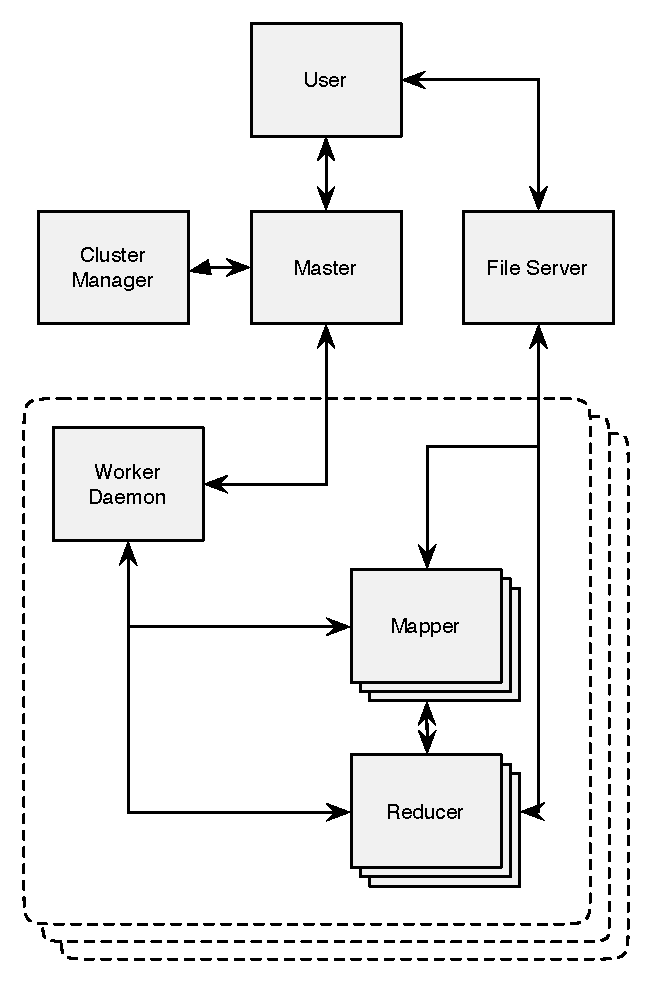
\includegraphics{Architecture.pdf}
}
\caption{The major components found in our architecture.}
\label{fig:arch}
\end{center}
\end{figure}


Our proposed architecture is shown in Figure~\ref{fig:arch}. We first describe the major difference between our proposed architecture and the architecture suggested in prior implementations of MapReduce. We then explain our architecture and the RPCs it uses to communicate by taking the reader through the running of a typical MapReduce job. We finish this section by describing our mechanisms for tolerating faults and summarize the RPCs used in our architecture.

\subsection{Main difference}

The major difference between our architecture and prior implementations of MapReduce is that there is a worker daemon that sits on each node that mediates all communication between the master and the worker---including RPCing intermediate key/values to the reducers. This has some advantages and disadvantages.

There are three advantages to this approach. The first is that mapper threads can free system resources by closing immediately upon completion. This is especially important in systems where memory is scarce. This property has a secondary advantage: it entirely removes a failure case. Jobs no longer need to be rerun if mappers crash after completion since the daemon is responsible for all RPC with the reducers. Additionally, since worker communication is centralized by the daemon we can reduce network overhead by batching messages.

The principle disadvantage of the daemon approach is that the worker daemon takes the node down when it crashes.  Essentially, a node is removed from the MapReduce pool if the daemon crashes. However, since the daemon is isolated from the user's code and data we expect this to be a somewhat rare event.

We feel that this design decision is reasonable for a MapReduce implementation that is intended for memory-constrained systems.

\subsection{Typical Use}

So how does a typical MapReduce job look on this system? The sequence is initiated by the user when he contacts the master process and submits a MapReduce job using the \rpc{SubmitJob} RPC, which the user will block on\footnote{This is the only synchronous RPC call  that we will use.}. In the initial version of our system we will assume that there is a single well-known master that is always available and that failures of the master are catastrophic. The user provides, in this initial RPC, the location of programs that carry out the \emph{map} and \emph{reduce} operations. At this point in the design, we expect these programs to be precompiled executables located in the DFS.

After receiving this initial message the master requests that the worker daemon on each node start \emph{mapper} threads with \rpc{StartMapper}. The master will try to place \emph{map} jobs on nodes that already have a replicated copy of the appropriate split of the input data.  We assume in this phase of the work that the user has access to the complete cluster and that the current MapReduce job is the only job running on the system. Later iterations of our work will have to include interactions with a cluster resource manager. We also assume that the worker daemons are already running on the worker nodes.

The worker daemon, upon receipt of a \emph{map} work request, spawns a new \emph{mapper} thread for each request it gets. Because the worker daemon never delays or rejects any work request the master is completely responsible for work scheduling. The  \rpc{StartMapper} call includes a list of input chunks from the DFS. For now, we will assume that each chunk belongs to a single file and that we do not have to worry about the boundaries of multi-chunk files---\textit{e.g.} if a text document spans two chunks a word does not start in one block and end in another.

The \emph{mapper} thread buffers and writes the intermediate key-value pairs to local disk. Upon completion of the job, the mapper informs the worker daemon that it is done with \rpc{ReportLocalWorkComplete}, and exits. The worker daemon then contacts the master with \rpc{ReportWorkComplete} to inform it that it has some finished work.

In response to the finished work the master may initiate some new \emph{reducer} threads with \rpc{StartReducer}. When all the necessary \emph{mappers} exit, the master informs the corresponding \emph{reducers} that they have new work with \rpc{ReportNewWork}. If the intermediate key/values  are local then the \emph{reducer} can read them right from disk. If not, then the key/values are requested from the remote worker daemon with a \rpc{SendData} call. All of the intermediate data is read before the \emph{reducer} starts executing the user's \emph{reduce} code.

While running the user's code the \emph{reducer} thread writes the final key/value pairs to a temporary local file. Upon completion the \emph{reducer} atomically writes this local file to the DFS and sends the worker daemon the \rpc{ReportLocalWorkComplete}. The worker daemon forwards this to the master by the \rpc{ReportWorkComplete} call.

\subsection{Fault Tolerance}
The above process needs to be resilient to machines and threads failing. We will tolerate worker nodes, worker threads, and worker daemons crashing. We will not tolerate the master failing.

We use a `checking in' model to keep track of the dispatched jobs which saves the master from having to actively query the status of the workers. Whenever a mapper or a reducer is working, it will occasionally report to their associated worker daemon with \rpc{LocalCheckIn}. Less frequently, the worker daemon will send the master a list of jobs that have not reported in recently with \rpc{CheckIn}. On a node with all threads reporting normally the list will be empty.

If a job has not checked in for a while (\textit{i.e.} has been on the worker daemon's non-responsive list for some number of reports) then the master will reschedule it: it will send a \rpc{Kill} to the worker daemon for that job and dispatch a new request for work. Notice that because the worker daemon is responsible for sending data to the \emph{reducers}, we do not need to notify any \emph{reducers} about failed \emph{mappers}.

If the entire node goes down (\textit{i.e.} the worker daemon has not checked in for a while), then the master sends a \rpc{Kill} to the worker daemon for all of its jobs, then \rpc{ReportFail}'s any reducer that depends on mappers on that node. Finally, the master reschedules all work on the downed node.

%\citet{dean04mapreduce}

\subsection{RPC calls}

Here is a summary of the RPC calls used in our system:

\begin{table}[htdp]
\caption{Stored procedures on the master.}
\begin{center}
\resizebox{0.9\columnwidth}{!}{
\begin{tabular}{|l|l|}\hline
\textbf{Procedure} & \textbf{Arguments}\\\hline
\rpc{SubmitJob} & Input Directory, Output Directory, \\
&\qquad Map Program, Reduce Program, R, M\\
\rpc{CheckIn} & WorkerID, JobID List\\
\rpc{ReportWorkComplete} & WorkerID, JobID\\\hline
\end{tabular}
}
\end{center}
\label{default}
\end{table}%

\begin{table}[htdp]
\caption{Stored procedures on the worker daemon}
\begin{center}
\resizebox{0.9\columnwidth}{!}{
\begin{tabular}{|l|l|}\hline
\textbf{Procedure} & \textbf{Arguments}\\\hline
\rpc{StartMapper} & JobID, DFS chunk list \\
\rpc{StartReducer} & JobID, Key, OutputFile \\
\rpc{ReportLocalWorkComplete} & JobID\\
\rpc{ReportNewWork} & Mapper IP, Mapper JobID\\
\rpc{ReportFail} & Mapper IP, Mapper JobID\\
\rpc{SendData} & JobID, Key\\
\rpc{Kill} & JobID\\
\rpc{LocalCheckIn} & JobID\\\hline
\end{tabular}
}
\end{center}
\label{default}
\end{table}%



\section{Milestone Deliverables}
We plan to prototype the architecture in C++ using the Apache Thrift framework for implementing RPCs. We will use the prototype to test and study how different design decisions affect the performance of MapReduce. After identifying them we will fine tune our final implementation for optimal memory, power, and network usage.


\bibliographystyle{plain}
\bibliography{references}


\end{document}
